\documentclass{beamer}
\beamertemplatenavigationsymbolsempty
\usecolortheme{beaver}
\setbeamertemplate{blocks}[rounded=true, shadow=true]
\setbeamertemplate{footline}[page number]
%
\usepackage[utf8]{inputenc}
\usepackage[english,russian]{babel}
\usepackage{amssymb,amsfonts,amsmath,mathtext}
%\usepackage{subfig}
\usepackage[all]{xy} % xy package for diagrams
\usepackage{array}
\usepackage{multicol}% many columns in slide
\usepackage{hyperref}% urls
\usepackage{hhline}%tables
\usepackage{wrapfig}
% Your figures are here:
\graphicspath{ {fig/} {../fig/} }
\usepackage{subfigure}
\newtheorem{assumption}{Assumption}
\setbeamertemplate{theorems}[numbered]
%\setbeamertemplate{caption}[numbered]

%----------------------------------------------------------------------------------------------------------
\title[\hbox to 56mm{\href{https://arxiv.org/pdf/2003.01227}{Laplace Bridge}}]{\href{https://arxiv.org/pdf/2002.03495}{Laplpace Bridge}}
\author[Ignashin Igor]{Ignashin Igor}
\institute{Bayesian multimodeling \\
Department of Intelligent Systems, MIPT}
\date{December 2024}

%----------------------------------------------------------------------------------------------------------
\begin{document}
%----------------------------------------------------------------------------------------------------------
\begin{frame}
\thispagestyle{empty}
\maketitle
\end{frame}
%-----------------------------------------------------------------------------------------------------
\begin{frame}{Laplace approximation}
\footnotesize
\begin{gather*}
    p(\theta | D) := \frac{1}{Z} p(D | \theta) p(\theta) \\
    p(D | \theta) p(\theta) =: h(\theta) \\
    Z = \int \exp(\log h(\theta)) d\theta \\ 
    \theta_{\text{MAP}} := \arg \max_\theta \log p(\theta | D) = \arg \max_\theta \log h(\theta) \\ 
    \log h(\theta) \approx \log h(\theta_{\text{MAP}}) - \frac{1}{2} (\theta - \theta_{\text{MAP}})^{\top} \Lambda (\theta - \theta_{\text{MAP}}) \\    
    \Lambda := -\nabla^2 \log h(\theta) \big|_{\theta = \theta_{\text{MAP}}} \\
    Z \approx \exp(\log h(\theta_{\text{MAP}})) \int \exp \left( -\frac{1}{2} (\theta - \theta_{\text{MAP}})^{\top} \Lambda (\theta - \theta_{\text{MAP}}) \right) d\theta = \\
    = h(\theta_{\text{MAP}}) \left( \frac{(2\pi)^{d/2}}{(\det \Lambda)^{1/2}} \right) \\ 
    p(\theta | D) = \frac{1}{Z} h(\theta) \approx \frac{(\det \Lambda)^{-1/2}}{(2\pi)^{d/2}} \exp \left( -\frac{1}{2} (\theta - \theta_{\text{MAP}})^{\top} \Lambda (\theta - \theta_{\text{MAP}}) \right),
\end{gather*}
 Which we can immediately identify as the Gaussian density $\mathcal{N}(\theta | \theta_{\text{MAP}}, \Sigma)$ with mean $\theta_{\text{MAP}}$ and covariance matrix $\Sigma := \Lambda^{-1}$.

\end{frame}

%-----------------------------------------------------------------------------------------------------------
\begin{frame}{Dirichle distribution}
The Dirichlet distribution, which has the density function:
\begin{gather*}
    \text{Dir}(\pi | \alpha) := \frac{\Gamma\left(\sum_{k=1}^{K} \alpha_k\right)}{\prod_{k=1}^{K} \Gamma(\alpha_k)} \prod_{k=1}^{K} \pi_k^{\alpha_k - 1}, \quad (1)
\end{gather*}
Is defined on the probability simplex and can be “multimodal” in the sense that the distribution diverges in the \( k \)-corner of the simplex when \( \alpha_k < 1 \). 

This implies the incorrectness of applying the Laplace approximation to this distribution, because the approximation is unimodal.

\end{frame}

%-----------------------------------------------------------------------------------------------------------
\begin{frame}{Change of variable }

However, MacKay [1998] noted that both can
be elegantly corrected by changing the variable.

Consider the \( K \)-dimensional variable \( \pi \sim \text{Dir}(\pi | \alpha) \) defined as the softmax of \( z \in \mathbb{R}^K \):

\begin{gather*}
    \pi_k(z) := \frac{\exp(z_k)}{\sum_{l=1}^{K} \exp(z_l)}, \quad \text{for all } k = 1, \ldots, K.
\end{gather*}

We will call \( z \) the logit of \( \pi \). When expressed as a function of \( z \), the density of the Dirichlet in \( \pi \) has to be multiplied by the absolute value of the determinant of the Jacobian:

\begin{gather*}
    J = \det \left( \frac{\partial \pi}{\partial z} \right) = \prod_{k} \pi_k(z_k).
\end{gather*}
\end{frame}

%-----------------------------------------------------------------------------------------------------------

\begin{frame}{Laplace Bridge}
\footntesize
After multiplying by the Jacobian:
\begin{gather*}
    \text{Dir}_z(\pi(z) | \alpha) := \frac{\Gamma\left(\sum_{k=1}^{K} \alpha_k\right)}{\prod_{k=1}^{K} \Gamma(\alpha_k)} \prod_{k=1}^{K} \pi_k(z)^{\alpha_k}.
\end{gather*}

This density of \( z \), the Dirichlet distribution in the softmax basis, can now be accurately approximated by a Gaussian through a Laplace approximation. 

Analytic map from the parameter \( \alpha \in \mathbb{R}^K_+ \) to the parameters of the Gaussian (\( \mu \in \mathbb{R}^K \) and symmetric positive definite \( \Sigma \in \mathbb{R}^{K \times K} \)), given by:
\begin{gather*}
    \mu_k = \log \alpha_k - \frac{1}{K} \sum_{l=1}^{K} \log \alpha_l \\
    \Sigma_{k\ell} = \delta_{k\ell} \left( \frac{1}{\alpha_k} - \frac{1}{K} \left( \frac{1}{\alpha_k} + \frac{1}{\alpha_\ell} - \frac{1}{K} \sum_{u=1}^{K} \frac{1}{\alpha_u} \right) \right).
\end{gather*}
\end{frame}

%-----------------------------------------------------------------------------------------------------------
\begin{frame}{Inverse map}

A pseudo-inverse of this map was provided as a side result
in Hennig et al. [2012]. It maps the Gaussian parameters to
those of the Dirichlet as

\begin{equation}
\alpha_k = \frac{1}{\Sigma_{kk}} \left( 1 - \frac{2}{K} + e^{\mu_k} \sum_{l=1}^{K} e^{-\mu_l} \right)
\end{equation}

This equation ignores off-diagonal elements of $\Sigma$.

This and the previous 2 equations will be called the Laplace Bridge. 

For Bayesian deep learning, only this equation is used, which displays values from $\mu$, $\Sigma$ to $\alpha$.

Despite the fact that LB implies a decrease
in the expressiveness of the distribution, however, the display is still quite accurate.

\end{frame}


%-----------------------------------------------------------------------------------------------------------
\begin{frame}{Visualization Laplace bridge }     
    \begin{figure}
        \centering
        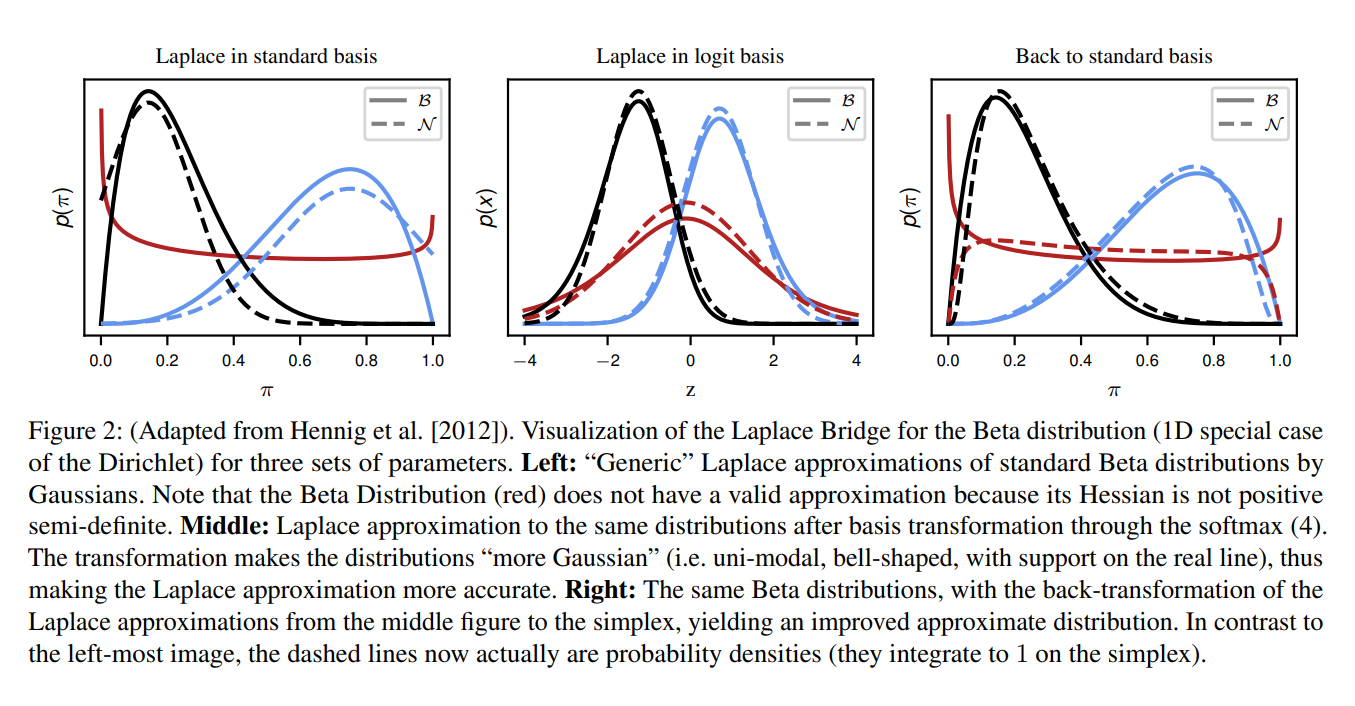
\includegraphics[width=1.0\textwidth]{figs/beta.png} % Путь к файлу изображения
    \end{figure}
\end{frame}

%-----------------------------------------------------------------------------------------------------------


\begin{frame}{Softmax in NN}
    \begin{figure}
        \centering
        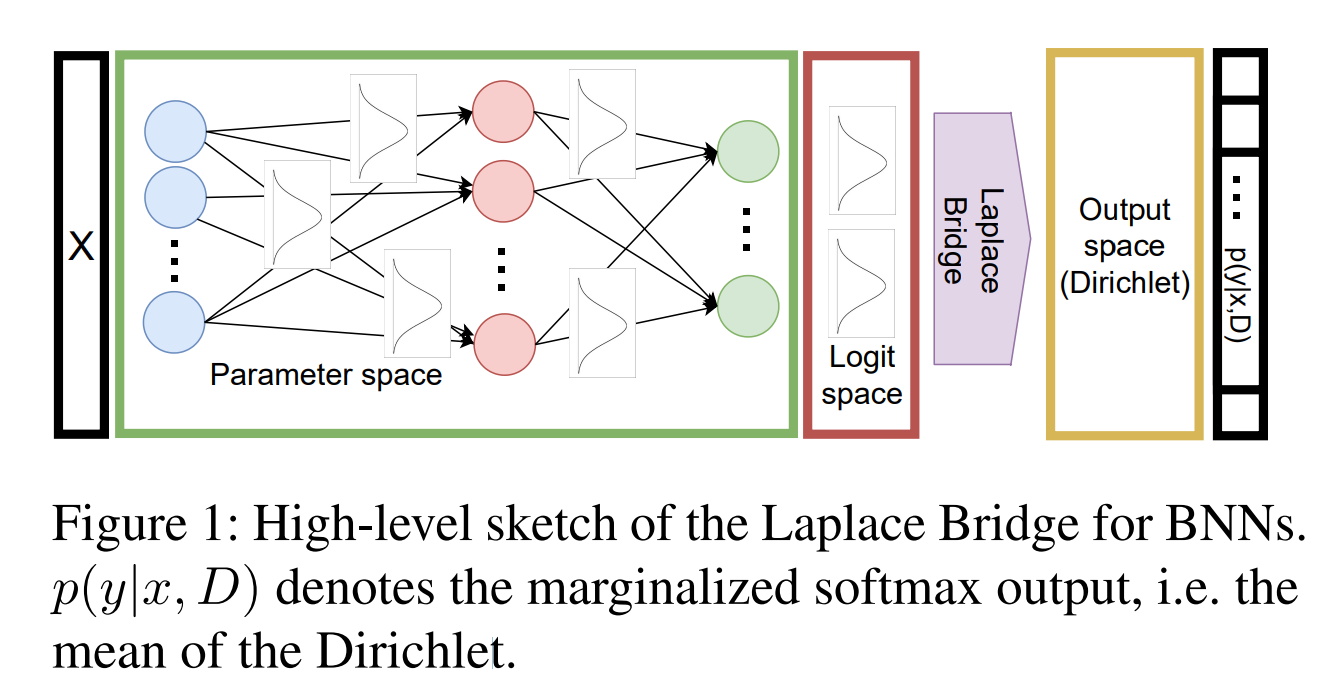
\includegraphics[width=1.0\textwidth]{figs/softmax.png} % Путь к файлу изображения
    \end{figure}
\end{frame}


%-----------------------------------------------------------------------------------------------------------
\begin{frame}{Laplace Approximation in BNN}

The Laplace Bridge can be applied to any NN setup that
maps from a Gaussian to probabilities by using the softmax.

Consider a last-layer Laplace approximation of the network \begin{equation}
    q(z|x) \approx \mathcal{N} \left(z \big| \mu_{W(L)} \phi(x), \phi(x)^T \Sigma_{W(L)} \phi(x) \right), \tag{8}
\end{equation}
where $\phi(x)$ the output of the first $L - 1$ layers, $\mu_{W(l)}$ is the maximum a posteriori (MAP) estimate for the weights of the last layer, $\Sigma_{ W(l)}$ is the inverse of the negative loss Hessian w.r.t. $W(l)$, given by $\Sigma_{W(L)} = -(\nabla^2_{W(L)} L)^{-1}$
around the MAP estimate $W(L)$. 

\end{frame}


%-----------------------------------------------------------------------------------------------------------
\begin{frame}{Laplace Bridge in BNN}
Given a dataset \( D := \{(x_i, t_i)\}_{i=1}^D \) and a prior \( p(\theta) \), let the posterior over the parameter \( \theta \) of an \( L \)-layer network \( f_\theta \) be defined as:
\begin{gather*}
p(\theta|D) \propto p(\theta)p(D|\theta) = p(\theta) \prod_{(x,t) \in D} p(y = t|\theta, x), \tag{40}
\end{gather*}
Then we can get an approximation of the posterior \( p(\theta|D) \) by fitting a Gaussian \( \mathcal{N} (\theta|\mu_\theta, \Sigma_\theta) \) where:
\begin{gather*}
\mu_\theta = \theta_{\text{MAP}}, \\
\Sigma_\theta = \left(-\nabla^2_{|\theta_{\text{MAP}}} \log p(\theta|D)\right)^{-1} =: H^{-1}_\theta.
\end{gather*}
That is, we fit a Gaussian centered at the mode \( \theta_{\text{MAP}} \) of \( p(\theta|D) \) with the covariance determined by the curvature at that point. 

For example, prior \( p(\theta) \) is a zero-mean isotropic Gaussian \( \mathcal{N} (\theta|0, \sigma^2 I) \) and the likelihood function is the Categorical density:
\begin{gather*}
p(D|\theta) = \prod_{(x,t) \in D} \text{Cat}(y = t|\text{softmax}(f_\theta(x))).
\end{gather*}

\end{frame}




%-----------------------------------------------------------------------------------------------------------
\begin{frame}{Notes}
 \begin{figure}
        \centering
        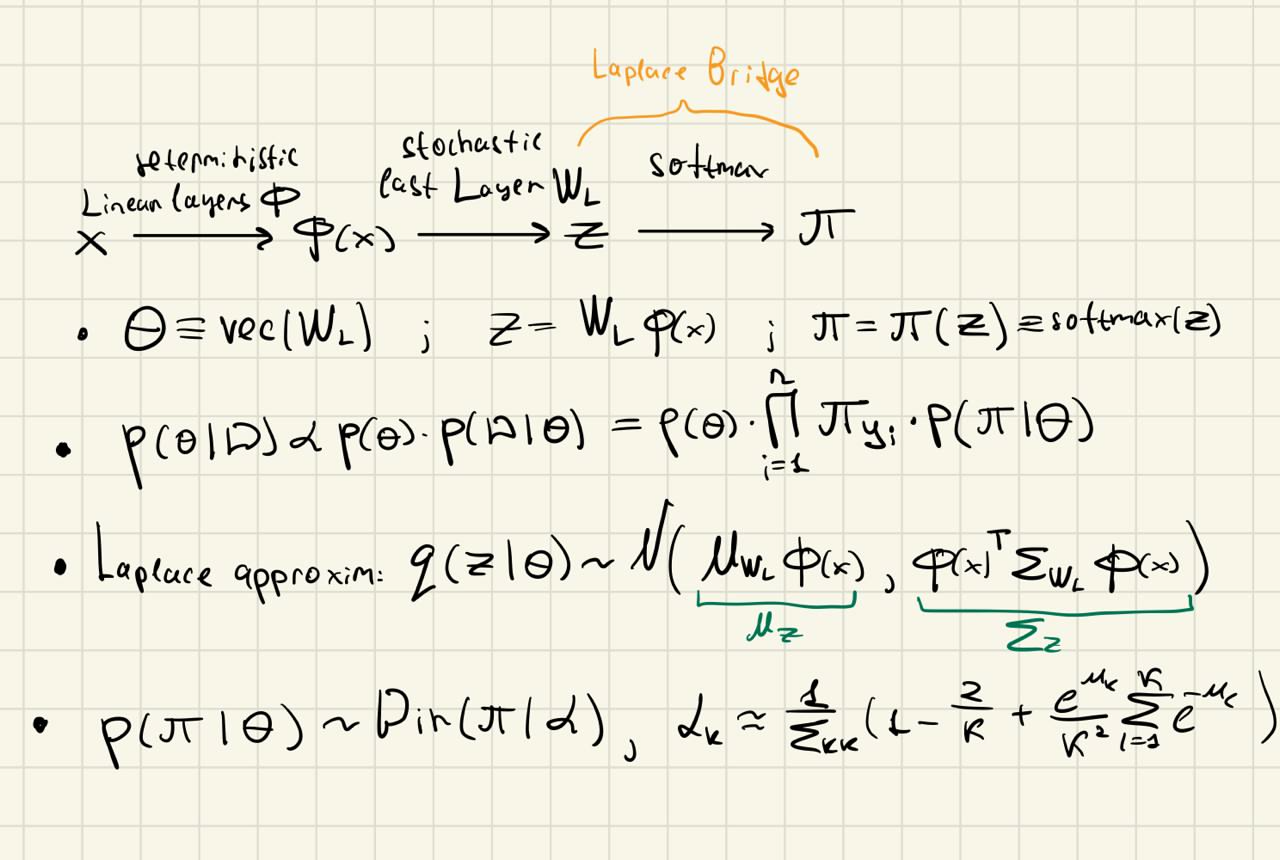
\includegraphics[width=1.0\textwidth]{figs/my.png} % Путь к файлу изображения
    \end{figure}

\end{frame}

%-----------------------------------------------------------------------------------------------------------

\begin{frame}{Limitations of LB}
 Two limitations of the LB: 
 \begin{itemize}
     \item First, the LB assumes that the random variable of the Gaussian sums to zero due to the difference in degrees of freedom between Dirichlet and Gaussian
 \end{itemize}  
 Thus, we have to add a correction that projects from any
arbitrary Gaussian to one that fulfills this constraint.
\begin{gather*}
    \mathcal{N} \left( x \big| \mu - \frac{\Sigma_{11}^T \mu}{1^T \Sigma_1}, \, \Sigma - \frac{\Sigma_{11} \Sigma_{1}^T}{1^T \Sigma_1} \right)
\end{gather*}
where \( 1 \) is the one-vector of size \( K \).
\end{frame}

%-----------------------------------------------------------------------------------------------------------

\begin{frame}{Limitations of LB}
\footnotesize
 \begin{itemize}
     \item Second, the softmax-Dirichlet distribution is asymmetric.
 \end{itemize}  
 \begin{figure}
        \centering
        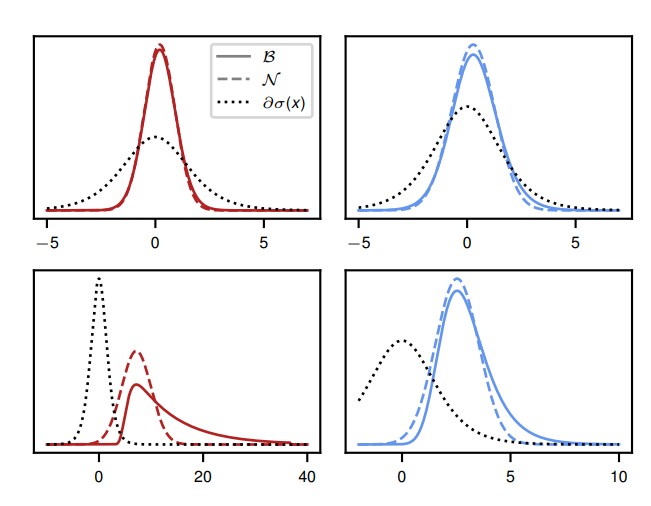
\includegraphics[width=0.7\textwidth]{figs/assymetric.png} % Путь к файлу изображения
    \end{figure}

\end{frame}

%-----------------------------------------------------------------------------------------------------------

\begin{frame}{Second correction}
\footnotesize
Autors propose an additional correction for practical purposes:

\[
c = v_{\text{mean}}(\Sigma) \cdot \frac{1}{\sqrt{K/2}}
\]

\[
\mu_0 = \frac{\mu}{\sqrt{c}}
\]

\[
\Sigma_0 = \frac{\Sigma}{c}
\]
where \( v_{\text{mean}}(\Sigma) \) denotes the mean variance of \( \Sigma \), defined as \( v_{\text{mean}}(\Sigma) = \sum_i \Sigma_{ii} \). 
The factor of \( \sqrt{\frac{1}{K/2}} \) is added because authors founds that higher dimensionalities require less correction. 

This normalization, which can be understood as “pulling back” the distribution into a space where it is symmetric, has higher approximation quality. 

This correction is applied after the zero-sum constraint correction.

\end{frame}


%-----------------------------------------------------------------------------------------------------------

\begin{frame}{Experiments }
     \begin{figure}
        \centering
        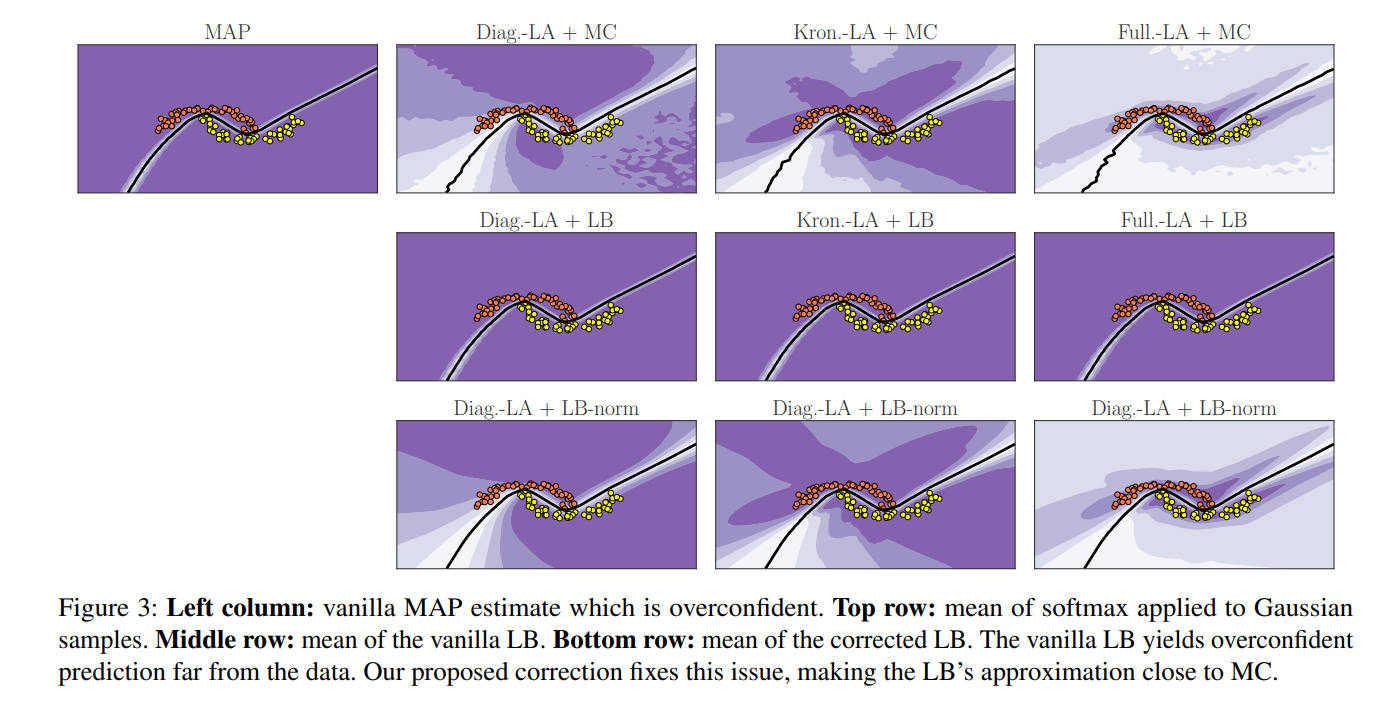
\includegraphics[width=1.1\textwidth]{figs/experiments.png} % Путь к файлу изображения
    \end{figure}
\end{frame}

%-----------------------------------------------------------------------------------------------------------
\begin{frame}{Inference}
 \begin{figure}
        \centering
        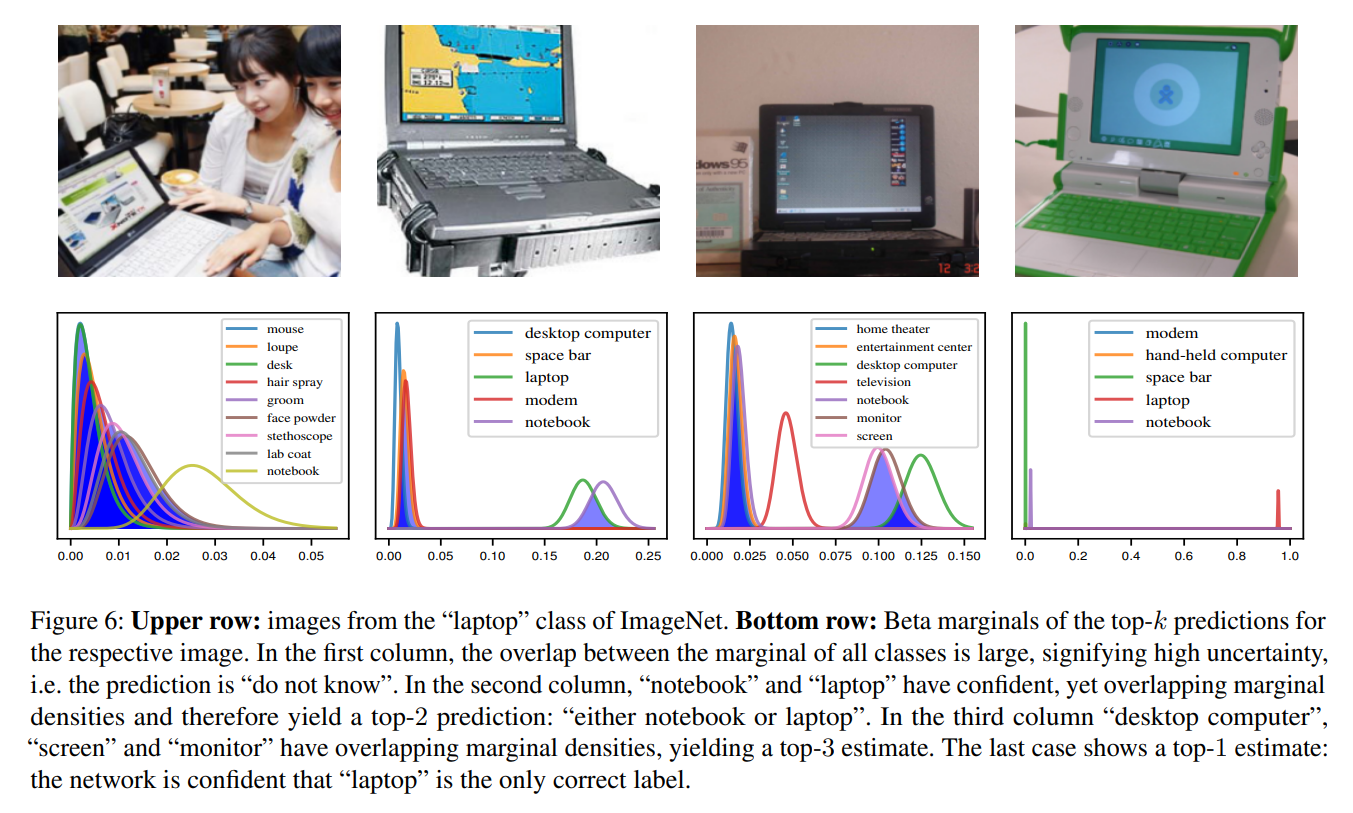
\includegraphics[width=1.0\textwidth]{figs/laptop.png} % Путь к файлу изображения
    \end{figure}

\end{frame}
%-----------------------------------------------------------------------------------------------------------
\begin{frame}{Conclusion}
    $\bullet$  Laplace Bridge analytically maps the marginal Gaussian prediction on logits to the Dirichlet distribution over softmax vectors.

    $\bullet$ Preservation of predictive uncertainty.

    $\bullet$ Significantly reduces the cost of predicting the posterior distribution in the testing phase while minimizing the cost increase in the training phase.

    $\bullet$ The vanilla Laplace Bridge method has some limitations, for which the author has proposed a simple correction that outperforms alternative approximations of the softmax integral.

\end{frame}

% \begin{frame}{Список литературы}
%     \footnotesize
%     \bibliographystyle{apalike}
%     \bibliography{refs}
% \end{frame}
%----------------------------------------------------------------------------------------------------------
\end{document} 